% ---------------------------------------------------------------------
% --- Arquivo principal e os demais serao os dos capitulos.
% --- EXPRESSÔES ENTRE <> DEVERÂO SER COMPLETADAS COM A INFORMAÇÂO ESPECÌFICA DO TRABALHO 
% ---------------------------------------------------------------------
\documentclass[ruledheader]{abnt_UFF}[abntex2]
\usepackage[alf]{abntex2cite}

%--- pacotes para hiphenizacao e acentuacao em portugues
\usepackage[brazil]{babel}
%\usepackage[latin1]{inputenc}
\usepackage[utf8]{inputenc}
\usepackage[T1]{fontenc}

%--- pacote para figuras
\usepackage{epsf}
\usepackage[dvips]{epsfig,graphicx}
\usepackage{subfigure}

%--- pacote de simbolos
\usepackage{latexsym}
\usepackage{textcomp}

%--- simbolos matematicos
\usepackage{amsmath}
\usepackage{amssymb}

%--- pacote para gerar pseudo-codigo
\usepackage{algorithm}
\usepackage{algorithmic}
\floatname{algorithm}{Algoritmo}

%--- outros pacotes
\usepackage{url}
\usepackage{longtable}
\usepackage{pdflscape}
\usepackage{setspace}
\usepackage{booktabs}
\usepackage{alltt}
\usepackage[flushleft]{threeparttable}
\renewcommand{\ttdefault}{txtt}

%Tabela Colorida
\usepackage{colortbl}
\usepackage{multicol}
\usepackage{multirow}
\usepackage{rotating}

\hyphenation{
    a-de-qua-da-men-te
    di-men-sio-na-men-to
}

%---------usando tipo de fonte padrao
\renewcommand{\ABNTchapterfont}{\bfseries\fontfamily{cmr}\fontseries{b}\selectfont}
\renewcommand{\ABNTsectionfont}{\bfseries\fontfamily{cmr}}

% --- -----------------------------------------------------------------
% --- Documento Principal.
% --- -----------------------------------------------------------------
% \usepackage[pdftex]{hyperref}
% \hypersetup{colorlinks, sitecolor=black, pdftex}

\begin{document}
    % --- Para elementos em português, remover.
    \renewcommand{\listfigurename}{Lista de Figuras}
    \renewcommand{\figurename}{Figura}
    \renewcommand{\listtablename}{Lista de Tabelas}
    \renewcommand{\tablename}{Tabela}
    \renewcommand{\contentsname}{Sumário}
    \renewcommand{\refname}{Referências}
    \renewcommand{\appendixname}{Apêndices}
    \renewcommand{\chaptername}{Capítulo}

% --- -----------------------------------------------------------------
% --- Titulo, abstract, dedicatorias e agradecimentos.
% --- Indice geral, lista de figuras e tabelas.
% --- -----------------------------------------------------------------
    	% --- -----------------------------------------------------------------
	% --- Elementos usados na Capa e na Folha de Rosto.
	% --- EXPRESS�ES ENTRE <> DEVER�O SER COMPLETADAS COM A INFORMA��O ESPEC�FICA DO TRABALHO
	% --- E OS S�MBOLOS <> DEVEM SER RETIRADOS 
	% --- -----------------------------------------------------------------
	\cleardoublepage
	\thispagestyle{empty}
	
	\vspace{-60mm}
	  \begin{singlespace}
	    \begin{center}
	      {\large UNIVERSIDADE FEDERAL DO ACRE}
	      \vskip4.0cm{\textbf{\Large Gustavo Moreira Oliveira de Castro}}
	      \vskip5.0cm {\textbf{Análise comparativa de estimadores monoculares de profundidade relativa}}
	    \end{center}
	    \begin{center}
	      \vskip10.0cm{\textbf{RIO BRANCO\\2024}}
	    \end{center}
	  \end{singlespace}
	% --- -----------------------------------------------------------------
	% --- Folha de rosto. (Obrigatorio)
	% --- ----------------------------------------------------------------
	\cleardoublepage
	\thispagestyle{empty}
	
	\vspace{-60mm}
	  \begin{center}
	    {\large UNIVERSIDADE FEDERAL DO ACRE}\\
	    \vspace{3cm}
	    {\large Gustavo Moreira Oliveira de Castro} \\
	    \vspace{3cm}
	    
	    {\large Análise comparativa de estimadores monoculares de profundidade relativa} \\
	    \vspace{1.5cm}
	  \end{center}
	
	\noindent
	  \begin{flushright}
	    \begin{minipage}[t]{8cm}
	     \textcolor{black}{Proposta de dissertação de mestrado submetida ao Programa de Pós-Graduação em Ciência da Computação na Universidade Federal do Acre como requisito parcial para obtenção do título de mestre em Ciência da Computação. Linha de Pesquisa: Sistemas Computacionais Inteligentes}
	    \end{minipage}
	  \end{flushright}
	
	\vskip1.50cm
	  \begin{center}
	    \small Orientador: \\
	    Prof. Dr. {Roger Fredy Larico Chavez}\vskip3.5cm 
	  \end{center}
	  \begin{center}
	    \vspace{4mm}
	    RIO BRANCO \\
	    %\vspace{6mm}
	    2024
	  \end{center}
	
	\thispagestyle{empty}
	% --- -----------------------------------------------------------------
	% --- Termo de aprovacao. (Obrigatorio)
	% --- ----------------------------------------------------------------
	\cleardoublepage
	\thispagestyle{empty}
	
	\vspace{-60mm}
	
	\begin{center}
	  {\large Gustavo Moreira Oliveira de Castro} \\
	  \vspace{7mm}
	
	  {\large Análise comparativa de estimadores monoculares de profundidade relativa} \\
	  \vspace{10mm}
	\end{center}
	
	\noindent
	\begin{flushright}
	  \begin{minipage}[t]{8cm}
	
		\textcolor{black}{Proposta de dissertação de mestrado submetida ao Programa de Pós-Graduação em Ciência da Computação na Universidade Federal do Acre como requisito parcial para obtenção do título de mestre em Ciência da Computação. Linha de Pesquisa: Sistemas Computacionais Inteligentes}.
	
	  \end{minipage}
	\end{flushright}
	
	\vspace{1.0 cm}
	\noindent
	
	Approved in <MONTH> of <YEAR>. \\
	\begin{flushright}
	  \parbox{11cm}
	  {
	    \begin{center}
	      \vspace{3mm}
	      \rule{11cm}{.1mm} \\
	      Prof. Dr. Roger Fredy Larico Chavez\\
	      Universidade Federal do Acre
	      \vspace{3mm}
	    \end{center}
     
     \begin{center}
	      \vspace{3mm}
	      \rule{11cm}{.1mm} \\
	      Prof. Dr. ...\\
	      Universidade Federal do Acre
	      \vspace{3mm}
	    \end{center}
     
     \begin{center}
	      \vspace{3mm}
	      \rule{11cm}{.1mm} \\
	      Prof. Dr. ...\\
	      Universidade Federal do Acre
	      \vspace{3mm}
	    \end{center}
	  }
	\end{flushright}
	
	\begin{center}
	  \vspace{4mm}
	  RIO BRANCO \\
	  %\vspace{6mm}
	  2024
	\end{center}
	
	% --- -----------------------------------------------------------------
	% --- Dedicatoria.(Opcional)
	% --- ----------------------------------------------------------------
	\cleardoublepage
	\thispagestyle{empty}
	\vspace*{200mm}
	
	\begin{flushright}
	  {\em
	dfsaas
	    \\
	   - 
	    \\ 
	    
	  }
	\end{flushright}
	\newpage
	
	% --- -----------------------------------------------------------------
	% --- Agradecimentos.(Opcional)
	% --- ----------------------------------------------------------------
	\pretextualchapter{Agradecimentos}
	\hspace{5mm}
	
	...
	
	% --- -----------------------------------------------------------------
	% --- Resumo em portugues.(Obrigatorio)
	% --- ----------------------------------------------------------------
	\begin{resumo}
	
	  \begin{center}{
	    \textbf{Análise comparativa de estimadores monoculares de profundidade relativa}}
	  \end{center}
	
	\begin{spacing}{1.0}
	  ...
	\end{spacing}
	{\hspace{-8mm} \bf{Palavras-chave}}: ...; ...; ...; ....
	
	\end{resumo}
	
	% --- -----------------------------------------------------------------
	% --- Resumo em lingua estrangeira.(Obrigatorio)
	% --- ----------------------------------------------------------------
	\begin{abstract}
	
	....
	
	{\hspace{-8mm} \bf{Keywords}}: Regression; GAMLSS; OLLST; Repeated measure in time
	
	\end{abstract}
	
	% --- -----------------------------------------------------------------
	% --- Lista de figuras.(Opcional)
	% --- -----------------------------------------------------------------
	%\cleardoublepage
	\listoffigures
	
	% --- -----------------------------------------------------------------
	% --- Lista de tabelas.(Opcional)
	% --- -----------------------------------------------------------------
	\cleardoublepage
	%\label{pag:last_page_introduction}
	\listoftables
	\cleardoublepage
	
	% --- -----------------------------------------------------------------
	% --- Sumario.(Obrigatorio)
	% --- -----------------------------------------------------------------
	\pagestyle{ruledheader}
	\tableofcontents
	
% --- -----------------------------------------------------------------
% --- Insercao dos capitulos.
% --- -----------------------------------------------------------------
    \pagestyle{ruledheader}
    \setcounter{page}{1}
    \pagenumbering{arabic}
    
\chapter{Introdução}

\section{Contextualização da pesquisa}

Informação de profundidade é uma das representações mais úteis para o entendimento de ambientes físicos \cite{lasinger2019towards} \cite{zhou2019does}. São também uma parte importante da caracterização de relações geométricas de uma determinada cena. As imagens de profundidades (ou mapas de profundidade) desempenham um papel importante em uma série de aplicações que envolvem visão computacional \cite{eigen2014depth}.  Entre elas, podemos citar: compreensão de cenas \cite{jaritz2018sparse}, veículos autônomos \cite{song2021self}, navegação de robôs \cite{ma2019sparse} navegação de VANTs, \cite{padhy2023monocular} fazendas inteligentes \cite{farkhani2019sparse}, e realidade aumentada \cite{du2020depthlab}. 

% \textit{Simultaneos Localization and Mapping} (SLAM) \cite{hu2012robust}

Os mapas de profundidade representam as distâncias de cada ponto (ou pixel) numa cena física em relação ao eixo do dispositivo de captura. Podem ser representados por imagens em escala de cinza, com as cores dos pixels sendo proporcionais à distância, com cinzas mais claros para objetos mais próximos e tons mais escuros para pontos mais afastados (e vice-versa) \cite{dourado2020multi}.

% \begin{figure}[h]
%     \centering
%     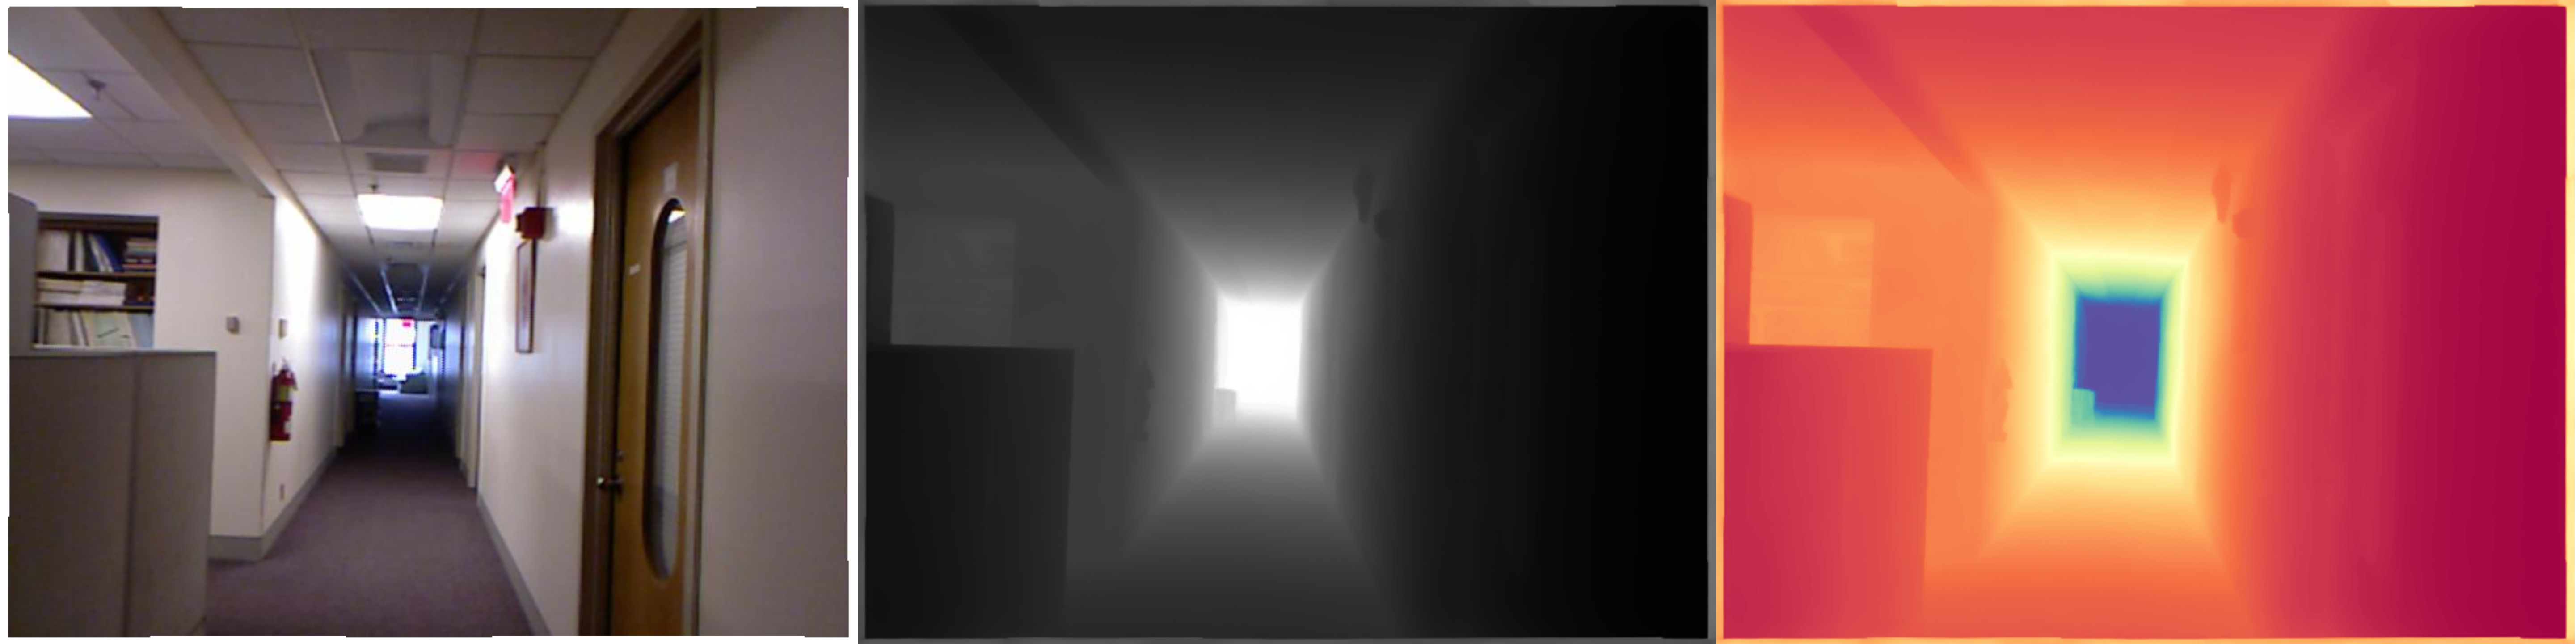
\includegraphics[width=\textwidth]{fig/example_depth.png}
%     \caption{Exemplo de mapa de profundidade do \textit{dataset Nyu Depth V2}. No primeiro quadro, a imagem RGB, no segundo, o mapa de profundidade em escala de cinza, no terceiro uma colorização artificial para o mapa de profundidade.}
%     \label{dmap}
% \end{figure}


Para capturar tais imagens geralmente são empregadas câmeras RGB-D, que podem prover tanto informação de profundidade quanto imagens coloridas da cena. Entre suas tecnologias mais comuns, são encontrados diversos tipos de aquisição que podem ser baseados em visão estereoscópica, que trabalha com múltiplos ângulos de visão, sensores \textit{Time-of-Flight} (ToF) que emprega projeção de lasers infravermelhos (IR) estruturados e técnicas mais precisas como o LiDAR (\textit{Light Detection and Ranging}) \cite{castellano2023performance}.


Sensores de profundidade estão cada vez mais embarcados em equipamentos amplamente difundidos como dispositivos de realidade aumentada (Occulus, Kinnect) e até mesmo em smartphones \cite{du2020depthlab}, principalmente as câmeras ToF, pois são capazes de desempenhar de maneira satisfatória mesmo com baixa potência \cite{branscombe2018microsoft}. De acordo com \cite{xie2021ultradepth}, a adoção de sensores de profundidade em smartphones tende a aumentar nos próximos anos, com diversas aplicações como tradução de linguagem de sinais \cite{park2021enabling} e sistemas de navegação mobile para pessoas com deficiência visual \cite{see2022smartphone}.

%sinal 57, gestos 86, e aumentada 97

Ainda segundo \cite{castellano2023performance}, cada uma das técnicas de aquisição de imagens de profundidade possui lados negativos que podem impactar os dados. Por exemplo, as câmeras ToF podem sofrer com invalidação de pixels próximos a cantos ou bordas de objetos devido à interferências entre os raios IR em superfícies descontínuas ou reflexivas \cite{hansard2012time}. Outros tipos de câmeras RGB-D mais comuns como o Microsoft Kinect ou Intel RealSense podem produzir valores inválidos em superfícies muito brilhantes ou reflexivas como espelhos, superfícies metálicas ou muito escuras \cite{zollhofer2019commodity}. Em ambientes internos, tais imagens podem conter até 50\% de dados faltantes. \cite{zhang2022indepth} \cite{zhang2018deep}. Pontos cuja medição é desconhecida são representados por pixels totalmente pretos ou totalmente brancos \cite{dourado2020multi}.

% \begin{figure}
%     \centering   
%     \includegraphics[width=\textwidth]{fig/depth_problema.png}
%     \caption{Exemplo de imagem RGB com mapa de profundidade apresentando leituras inválidas.}
%     \label{errdepth}
% \end{figure}

%problemas 27, 80, 98

Garantir a correta representação dos mapas em escala de pixel é de considerável importância para as tarefas que dependem de profundidade e que requerem um alto grau de segurança e confiabilidade dos dados, como veículos autônomos ou navegação de drones. A tecnologia LiDAR é a alternativa com implementação mais confiável entre as que foram citadas, no entanto, ressalta-se que nem o LiDAR e nem câmeras RGB-D convencionais produzem mapas completos e densos. No caso do LiDAR, são produzidos mapas esparsos (approx. 95\% de esparsidade) e no caso de câmeras RGB-D ou câmeras ToF são produzidos mapas com partes faltantes em determinadas superfícies ou bordas \cite{hu2012robust}. 




% Neste cenário, tecnologias de aquisição e melhoramento dos dados foram amplamente pesquisadas pela ciência nos últimos anos. Recentemente foram exploradas técnicas que não dependem de sensores de profundidade, ou seja, que inferem a informação de profundidade a partir de uma única imagem RGB capturada a partir de uma câmera comum, essa abordagem é conhecida como \textit{Monocular Depth Estimation} (MDE). No entanto, métodos baseados em características puramente visuais   \cite{szeliski2022computer} \cite{hu2022deep}. 



Considerando as limitações impostas por métodos ativos de aquisição de profundidade, surge a possibilidade de inferir um mapa de profundidade denso e completo de uma cena a partir de uma ou mais imagens RGB, processo conhecido como estimação de profundidade (\textit{Depth Estimation - DE}) \cite{rajapaksha2024deep}. Quando duas imagens de câmeras diferentes são utilizadas para obter-se a informação de profundidade, denomina-se \textit{Stereo Matching (SM)}. No entanto, métodos baseados em imagens \textit{stereo} requerem processos complexos de calibração e alinhamento \cite{dong2022towards}.


O problema da estimação monocular de profundidade (\textit{Monocular Depth Estimation - MDE}) tem por objetivo inferir o mapa de profundidade através de uma única imagem RGB. Esse problema é considerado mal-posto devido à ausência de informação geométrica na projeção da cena 3D para a imagem 2D. No entanto, os avanços nas tecnologias de \textit{Deep Learning - DL} e visão computacional tornaram factível e conveniente o uso de MDE para estimar mapas de profundidade densos e completos. \cite{spencer2024third} \cite{rajapaksha2024deep}. 

Ao longo dos anos, houveram diversas pesquisas científicas abordando o tema de estimação monocular de profundidade utilizando toda a miríade de técnicas e metodologias dentro do universo do DL, empregando desde redes neurais convolucionais \cite{kopf2021robust}, estruturas \textit{encoder-decoder} \cite{godard2019digging}, mistura de bases de dados em grande escala em modos diferentes \cite{lasinger2019towards}, transformadores de visão \cite{birkl2023midas}, modelos de difusão \cite{ke2024repurposing}, e treinamento utilizando dados reais pseudo-rotulados em larga escala \cite{yang2024depth}. 

Neste cenário, este trabalho propõe uma análise comparativa entre os diversos modelos de estimação monocular de profundidade relativa baseados em DL através da abordagem quantitativa, utilizando métricas e \textit{benchmarks} presentes na literatura, abordagem qualitativa e através de uma aplicação.



\section{Motivação e Justificativa} 


 
\section{Objetivos}


\subsection{Objetivo Geral}
Este trabalho possui como objetivo geral a análise comparativa de estimadores monoculares de profundidade robustos capazes de produzir informação de profundidade de alta qualidade para imagens sob quaisquer circunstâncias.

\subsection{Objetivos Específicos}

\begin{itemize}
    \item Estudo e escolha dos datasets que tenha as imagens apropriadas para teste.
    \item Estudo de modelos de estimação monocular de profundidade relativa do estado da arte.
    \item Análise e escolha entre os modelos estudados para implementação e testes.
    \item Implementação de método de pós-processamento para transferência do domínio relativo para métrico baseado em transformação de intensidade.
    \item Avaliação de desempenho perante métricas utilizadas na literatura para comparação entre os modelos no espaço relativo e métrico.
    \item Avaliação qualitativa dos resultados.
    \item Implementação de aplicação com os mapas de profundidade gerados.
    
\end{itemize}


    \chapter{Trabalhos Relacionados}



    


\chapter{Fundamentação Teórica}

\section{Processamento Digital de Imagens}

\section{Deep Learning}

\section{Informação de profundidade}

\section{Modelos de estimação de profundidade}

    
\chapter{Materiais e Métodos}

\section{Datasets}

Bases de dados para treinamento ou teste de algoritmos de estimação de profundidade consistem em imagens RGB de uma cena e sua anotação correspondente em profundidade. Ao longo do tempo, diversos \textit{datasets} foram propostos para este fim com variações em formatos de anotações, tipos de cena (interior ou exterior), métodos de captura, qualidade, resolução e tamanho.

% \textcolor{red}{colocar citações que tem na seção 3 do midas 1}.

Geralmente são empregados sensores e outras tecnologias como \textit{Stereo Matching} e \textit{Structure from Motion} para criar os \textit{datasets} de profundidade, porém, são abordagens muito complexas, custosas, ou inviáveis em algumas situações particulares, por exemplo, obter mapas de profundidades densos a partir de veículos em movimento  \cite{yang2024depthv1}.
Cada \textit{dataset} possui suas próprias características, problemas e viéses. Dados com informação de profundidade e em alta qualidade são complexos de adquirir, sendo que os melhores conjuntos são utilizados no treinamento dos modelos presentes na literatura \cite{ranftl2020towards}. 

Para avaliar os modelos de estimação de profundidade, será utilizado o protocolo de \textit{zero-shot cross-dataset transfer}, i.e. realizar os testes e métricas em bases de dados que não compuseram os conjuntos de treinamentos dos modelos analisados. A performance em \textit{cross-dataset} é considerada uma aproximação mais fiel da performance em mundo real em uma aplicação, pois os conjuntos de testes relativos aos conjuntos utilizados no treinamento podem refletir os mesmos viéses e situações \cite{ranftl2020towards}.

Dessa forma, para escolha das bases de dados a serem utilizadas para teste, temos os critérios: i) não ter composto o conjunto de treinamento dos modelos escolhidos para comparação, ii) conter dados válidos para avaliação considerando anotações precisas de profundidade, ou caso sejam esparsas, possuam máscara para indicar os pixels válidos, iii) ser uma base de dados conceituada na literatura. Os \textit{datasets} escolhidos e suas características podem ser visualizados na Tabela \ref{tabdata}.

% PESQUISA ANTIGA -------------------------------------------------------------------
% O presente trabalho exige um tipo de base de dados pouco encontrado na literatura, trios de imagem RGB, mapa de profundidade com erros e um outro mapa de profundidade denso e completo. De acordo com \cite{zhang2018deep}, uma das maneiras de se obter esses dados seria capturar imagens com uma câmera RGB-D de baixo custo e alinha-las com outra captura simultânea de um sensor mais preciso, porém essa abordagem é muito custosa, além de que não há disponibilidade de grandes conjuntos para treinamento.

% O presente projeto pretende utilizar como base de dados principal o \textbf{Hypersim}. Um \textit{dataset} para compreensão de cenas baseado em cenas sintéticas fotorrealistas. Contendo 77.400 imagens de 461 cenas \textit{indoor} com pares de RGB e mapas de profundidade calculado deterministicamente, além de outras informações como normais de superfície, rótulos de segmentação e detecção de objetos e entre outros \cite{roberts2021hypersim}.

% Please add the following required packages to your document preamble:
% \usepackage{graphicx}
\begin{table}[h]
    \centering
    \caption{Características dos datasets utilizados no trabalho}
    \label{tabdata}
    \resizebox{\textwidth}{!}{%
    \begin{tabular}{ccccccc}
    \hline
    \textbf{Dataset} & \textbf{Sensor} & \textbf{Anotação} & \textbf{Tipo} & \textbf{Cenário} & \textbf{Num. Imagens} & \textbf{Resolução} \\ \hline
    KITTI  & LiDAR         & Esparça & Real      & Outdoor        & 44 K   & 1024 $\times$ 320  \\
    Nyu-V2 & Kinect V1     & Densa   & Real      & Indoor         & 1449   & 640 $\times$ 480   \\
    DIODE  & Laser Scanner & Densa   & Real      & Indoor/Outdoor & 25,5 K & 768 $\times$ 1024  \\
    SINTEL & -             & Densa   & Sintético & Indoor/Outdoor & 1064   & 1024 $\times$ 436  \\
    ETH3D  & Laser Scanner & Densa   & Real      & Indoor/Outdoor & 454    & 6048 $\times$ 4032 \\ \hline
    \end{tabular}%
    }
    \end{table}


\subsection{NYUv2}


%% refazer o texto

O \textit{dataset} NYUv2 é um dos mais utilizados em tarefas de visão computacional que envolvam estimação de profundidade, segmentação de cenas e reconecimento de objetos. Possui 1449 pares de imagens RGB e mapas de profundidade densos em diversas cenas \textit{indoor} divididos em 795 para treinamento e 654 para teste \cite{silberman2012indoor}. A resolução das imagens é de 640 $\times$ 480 pixels. O equipamento de aquisição foi o equipamento Microsoft Kinect que utiliza a técnica de emissão de luz estruturada, que produz resultados precisos de informação de profundidade. Além dos pares RGB-D, também é disponibilizado os dados de leitura dos sensores puros em que é possível encontrar aproximadamente 70\% de pixels com informação válida de profundidade, no entanto, as imagens finais foram processadas utilizando um método de correção, resultando em um mapa denso, como observado na Figura \ref{exnyuv2}. Entre as cenas observadas no \textit{dataset}, podemos citar quartos, cozinhas, sala de aula, banheiro e etc. Além das informações de profundidade, a base de dados provém rótulos de segmentação de objetos e relações de suporte entre eles \cite{lahiri2024deep}.

\begin{figure}[h]
    \centering
    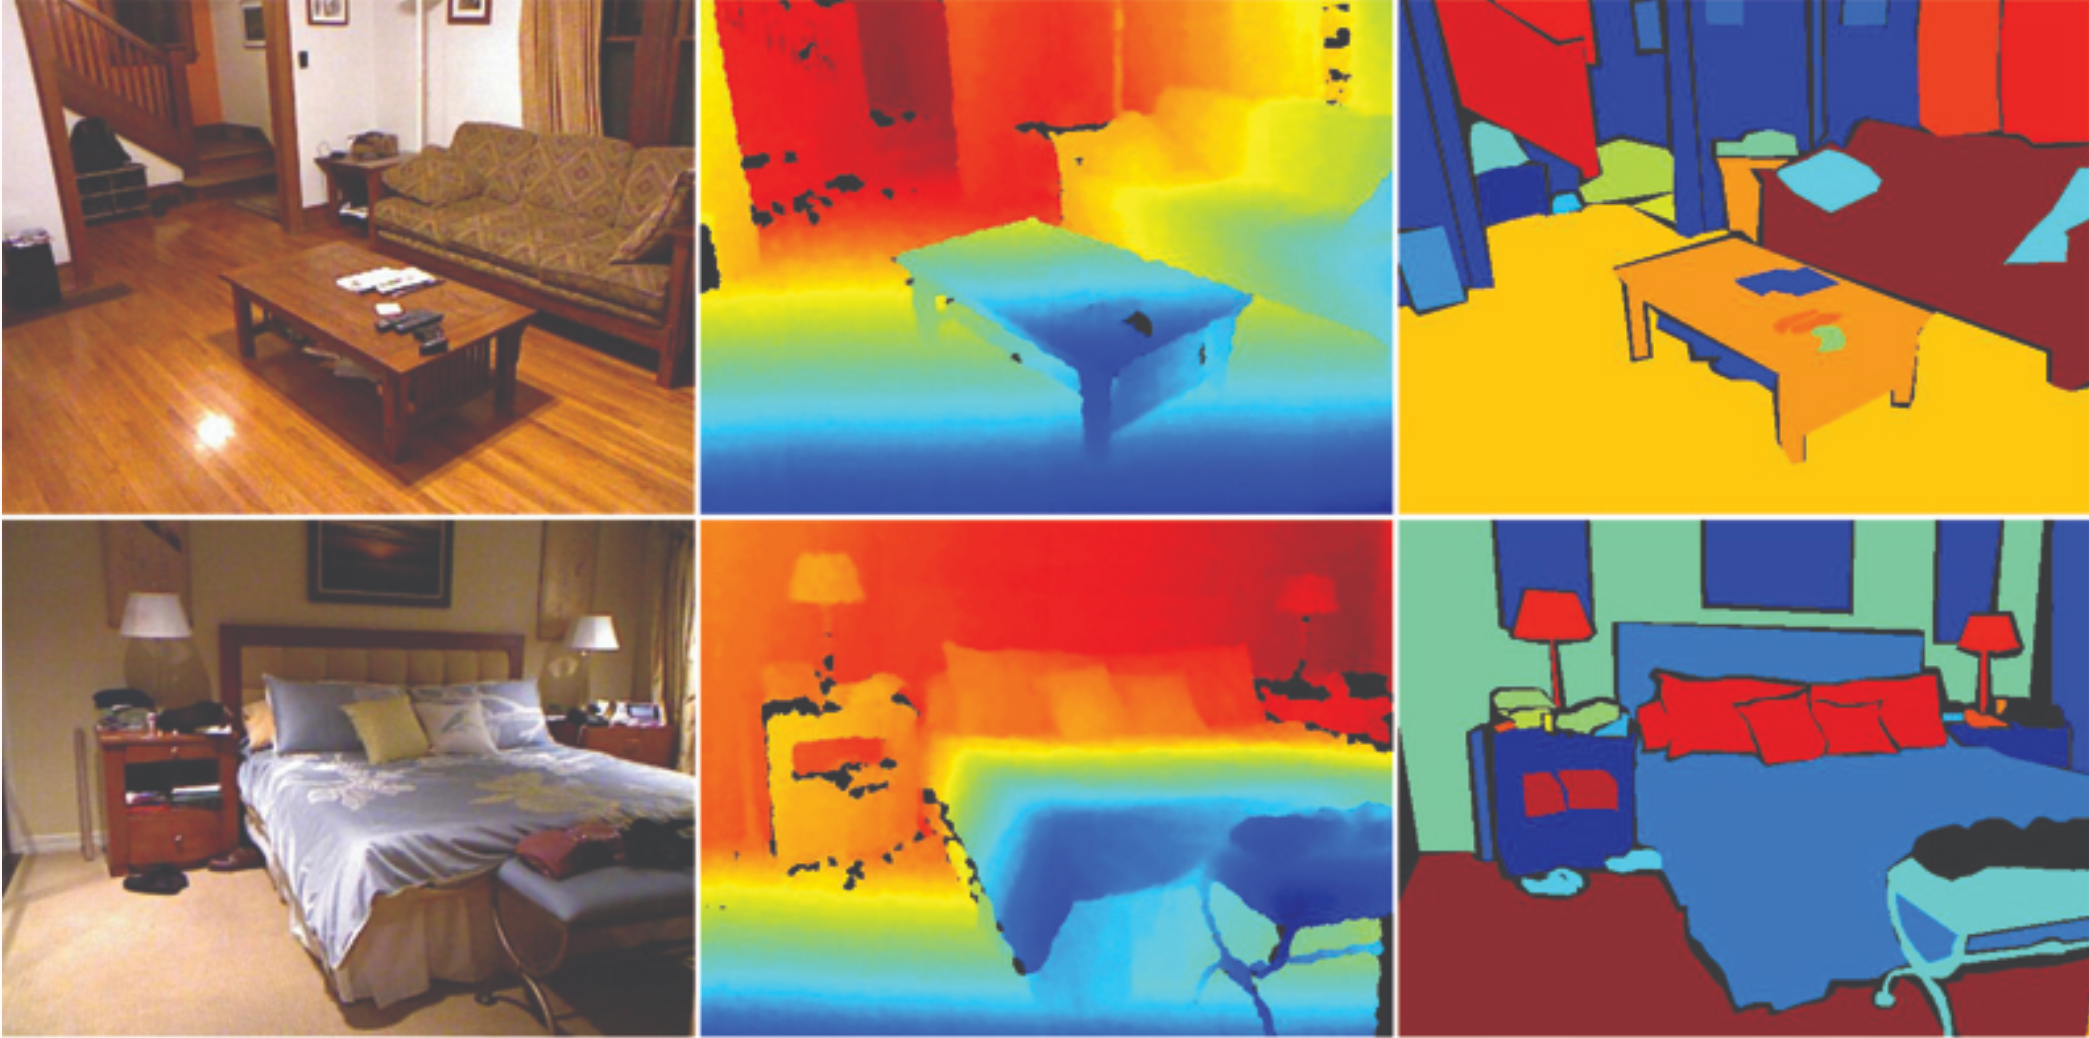
\includegraphics[width=\textwidth]{fig/example_nyu.png}
    \caption{Exemplo do dataset NYU Depth v2}
    \label{exnyuv2}
\end{figure}

\subsection{KITTI}



\subsection{SINTEL}

\subsection{ETH3D}

O ETH3D é uma base de dados geralmente utilizada para reconstrução em vistas múltiplas e \textit{stereo matching}. Contém dados de treinamento com imagens RGB \textit{multiview}, capturadas com câmeras DSLR e \textit{ground truth} de profundidade capturado utilizando um escâner a laser Faro Focus X 330. Oferece três versões de imagens de profundidade, uma correspondente à leitura bruta do sensor (\textit{raw}), outra com \textit{outliers} removidos por trabalho manual e uma ferramenta automática (\textit{clean}) e uma com \textit{outliers} e pontos observados por uma única imagem RGB removidos. A partição de teste não contém \textit{groundtruth}. A base de dados é associada à um desafio aberto ao público. Inclui cenas tanto internas quanto externas, oferecendo um protocolo de avaliação bem variado \cite{lahiri2024deep} \cite{schops2019bad}. 

\subsection{DIODE}

O \textit{dataset} DIODE (\textit{Dense Indoor and Outdoor Depth Dataset}), é uma base de dados para estimação monocular de profundidade e consiste em 8574+25 imagens de ambientes internos e 16.884+446 de ambientes externos para treinamento e teste. Possui resolução de 768 $\times$ 1024 com faixa de distâncias entre 50m e 300m para os ambientes internos e externos respectivamente. O equipamento de aquisição é o escâner a laser Faro Focus S350. Alguns exemplos do \textit{dataset} podem ser visualizados na Figura \ref{exdiode}.

\begin{figure}[h]
    \centering
    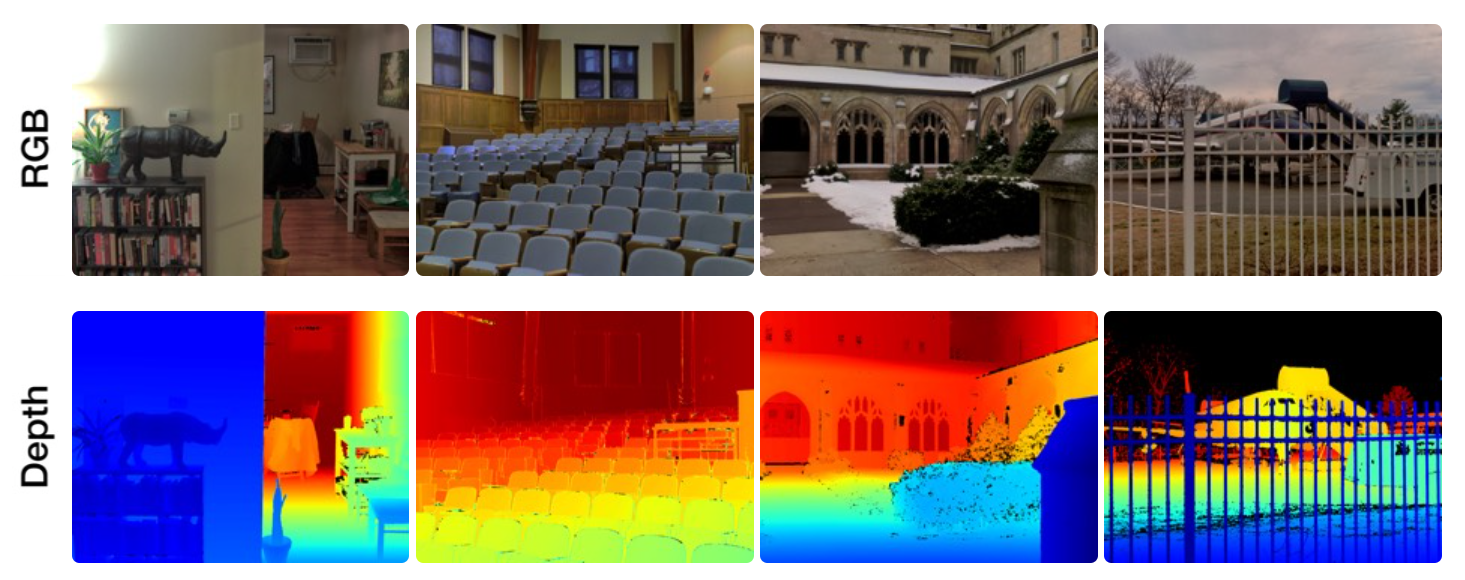
\includegraphics[width=\textwidth]{fig/example_diode.png}
    \caption{Exemplo do dataset DIODE}
    \label{exdiode}
\end{figure}

\section{Modelos Escolhidos}

\section{Protocolo de Avaliação}

\section{Método de Transformação de Intensidades (pós-processamento)}

Um mapa de profundidade inferido por um método de estimação de profundidade possui a característica de ser denso, pois todos os pixels possuem um valor predito associado, preciso, bem detalhado, de acordo com os últimos trabalhos do estado da arte porém é relativo, i.e. o valor de cada pixel é apenas correlacionado com a medição de distância real por um fator desconhecido. Já um mapa de profundidade adquirido com um sensor físico consegue representar as grandezas de forma métrica (em metros, centímetros ou até milimétros), mas pode ter características negativas associadas a depender do dispositivo de aquisição, podendo conter áreas falhas que não possuem medição associada, ou um elevado grau de esparsidade. O método de transformação de intensidades para transferência de domínio almeja como resultado uma imagem de profundidade que possuam as características positivas dos dois casos anteriormente citados. 

O método proposto por este trabalho consiste em uma transformação de intensidades que é projetada para cada imagem de um conjunto de dados utilizando pontos correspondentes em ambas e associando uma transformação linear para cada ponto, como visualizado na Figura \ref{posproc}. 


\begin{figure}[h]
    \centering
    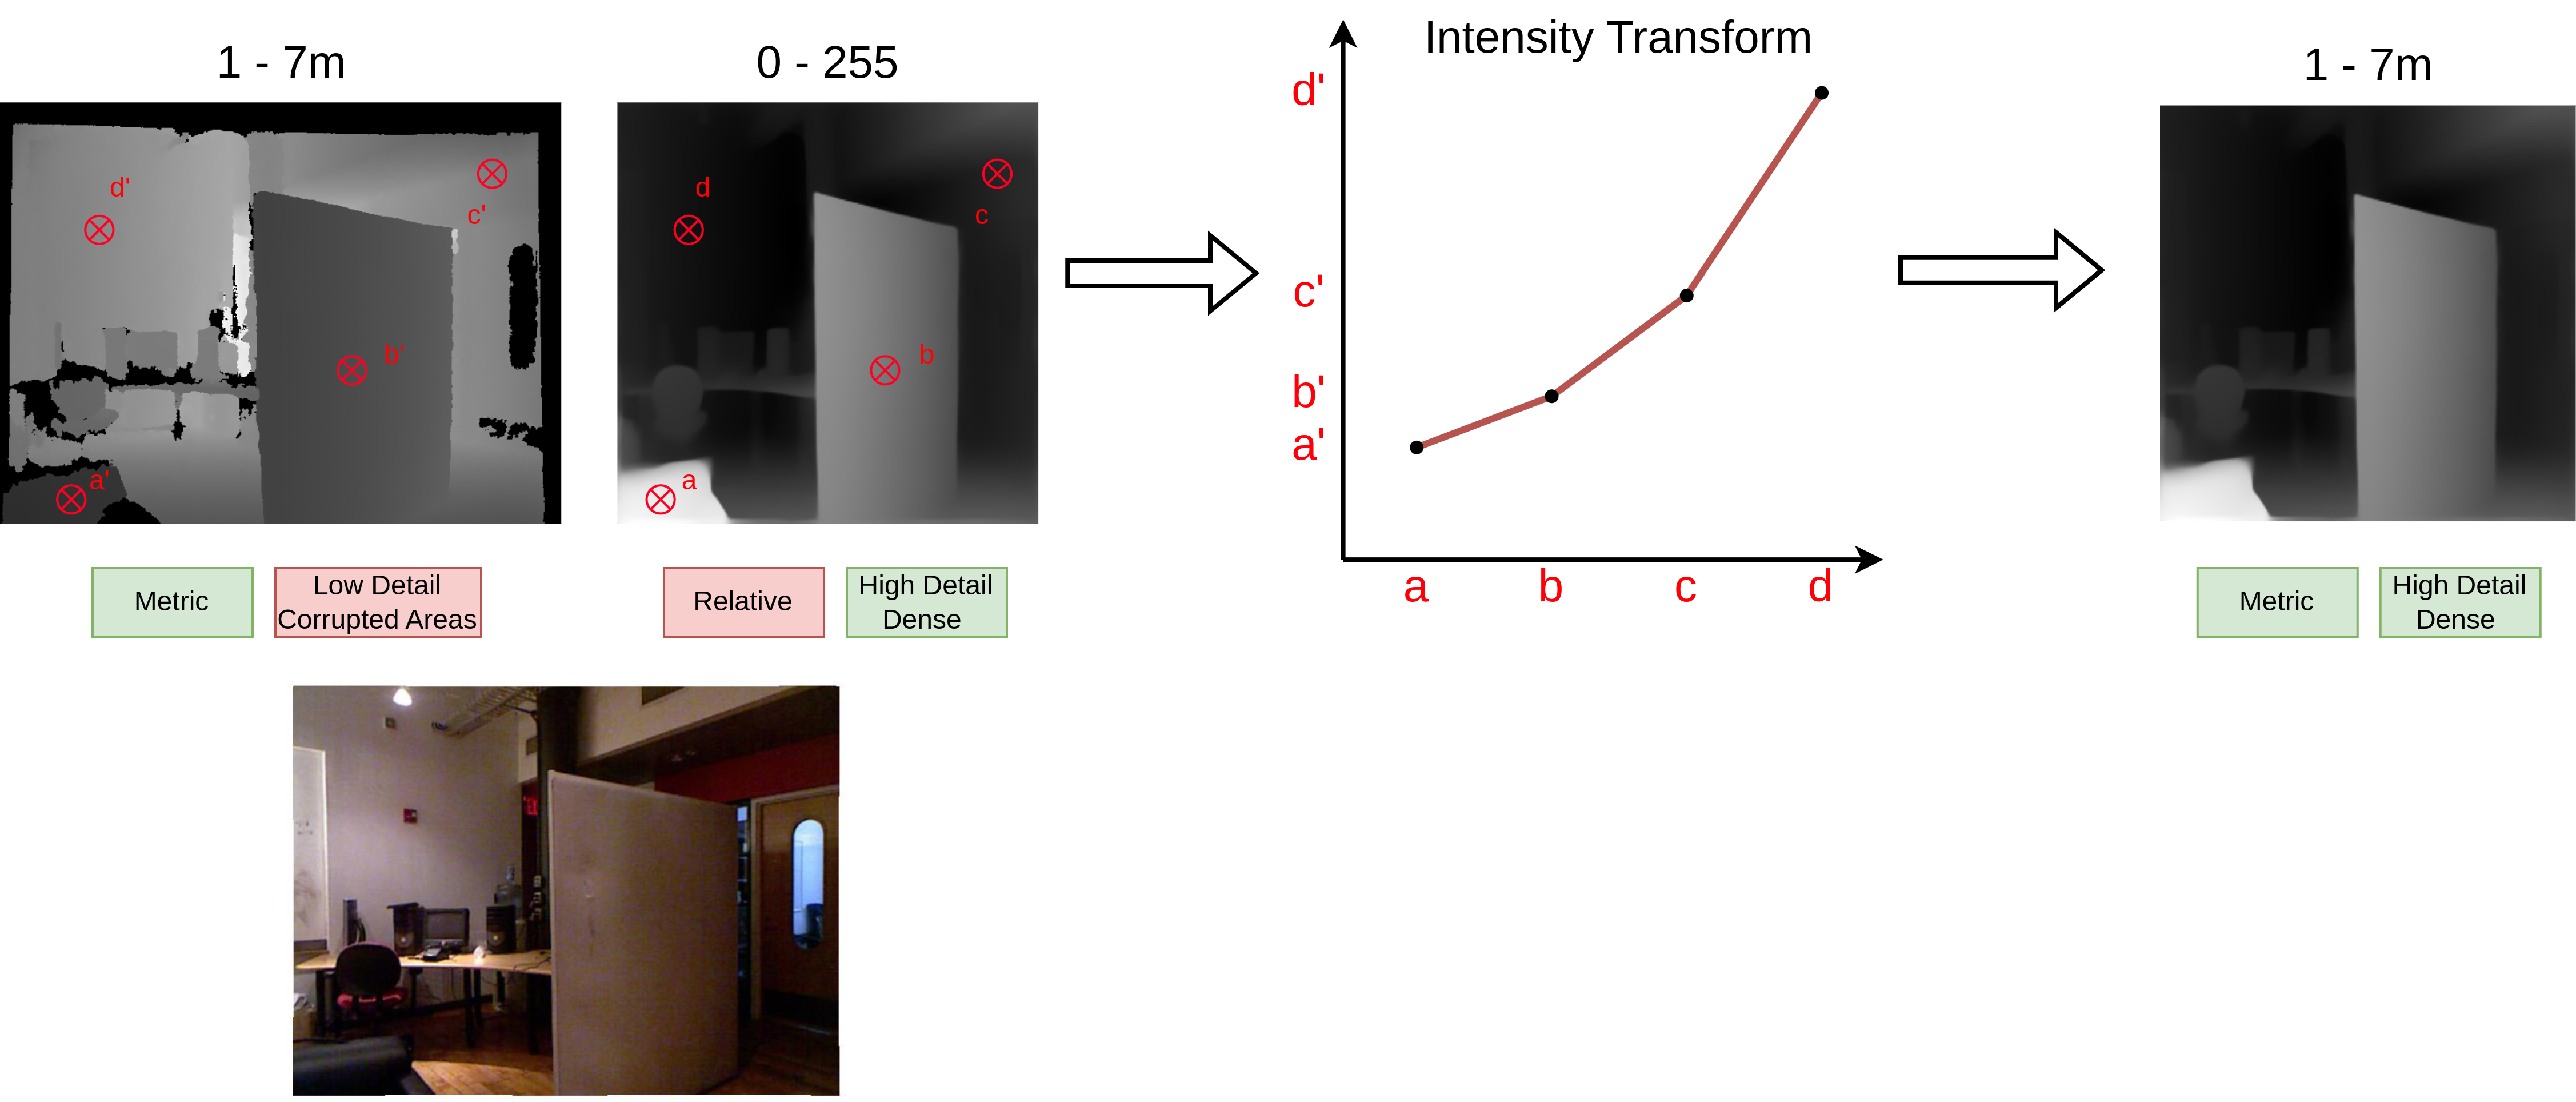
\includegraphics[width=\textwidth]{fig/diagram_normalization_white.png}
    \caption{Diagrama do método de transferência de domínio}
    \label{posproc}
\end{figure}

O método proposto diferencia-se do tradicional baseado em fator de escala e deslocamento por mínimos quadrados pois é associada uma função linear para cada região na quantização da imagem, o que propicia uma correção adaptada para cada proporção de distância. Ressalta-se que o método não será utilizado protocolo de avaliação dos modelos de estimação de profundidade, mas sim o que é mais prevalente na literatura.

Aos conjuntos de dados que possuem leituras métricas de sensores, será comparado o resultado da técnica de pós-processamento e o resultado de estimadores métricos de profundidade.

\section{Correção de mapas de profundidade} 

Para a tarefa de correção de mapas de profundidade utilizando redes neurais, o trabalho de \cite{hu2022deep} propôs duas categorias principais que se diferenciam pelos dados utilizados:

\begin{itemize}
    \item \textbf{Correção não-guiada} (Figura \ref{ung}): Objetiva completar diretamente as partes faltantes utilizando como entrada somente o mapa de profundidade.
    \item \textbf{Correção guiada} (Figura \ref{early} e \ref{late}): Objetiva completar as partes faltantes utilizando como entrada tanto o mapa de profundidade quanto a imagem RGB correspondente.
\end{itemize}

\begin{figure}[h]
    \centering
    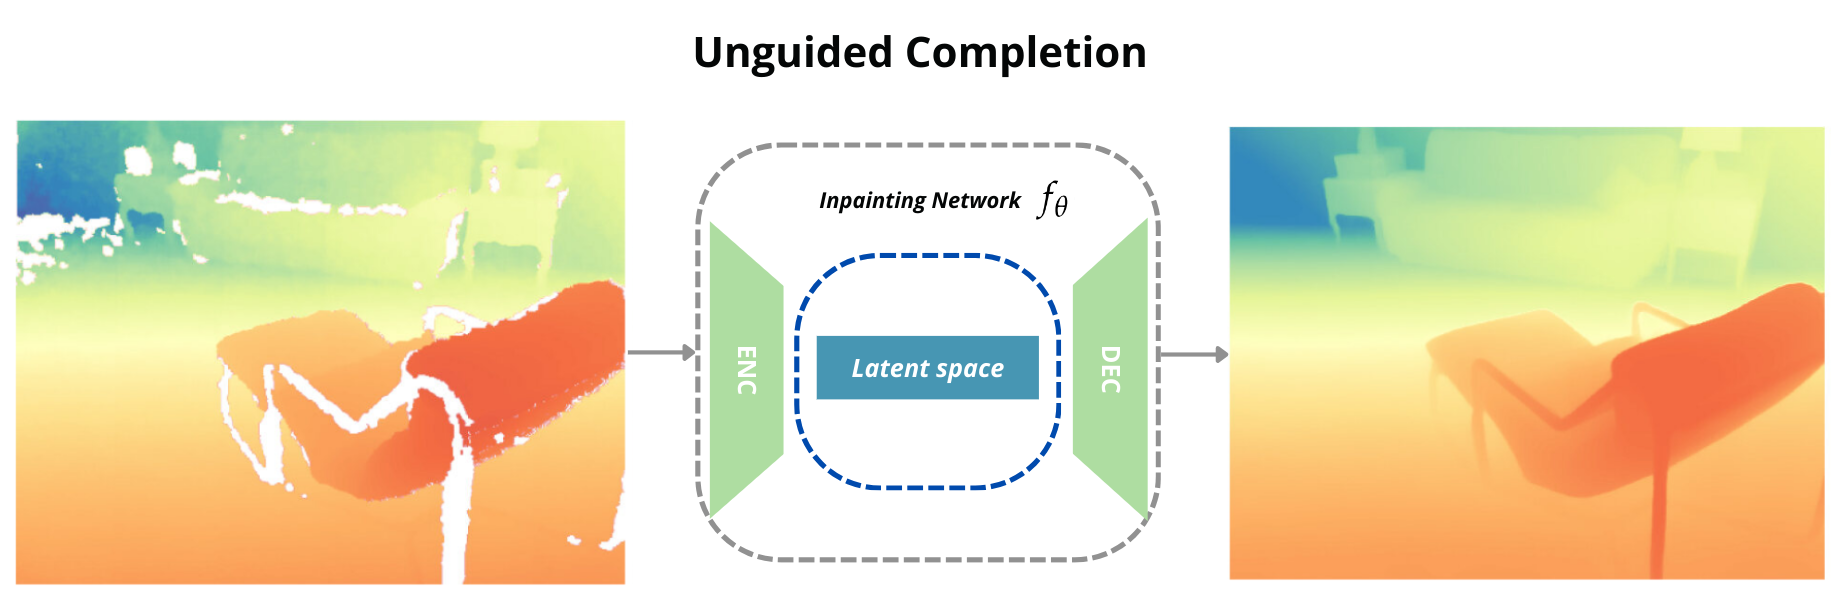
\includegraphics[width=\textwidth]{fig/unguided.png}
    \caption{Esquema de correção não-guiada.}
    \label{ung}
\end{figure}

A escolha da categoria de correção depende da quantidade de erros nas imagens. Quando há uma pequena quantidade de pixels inválidos, a correção não-guiada pode ser adequada, visto que não é necessário uma profunda extração de características dos dados. No entanto, no caso contrário, o uso de métodos guiados é indicado dado que existam grandes regiões com ausência de informação de profundidade ou que o mapa apresente uma grande esparsidade. Sendo necessário recorrer a extração dos atributos presentes na imagem RGB como bordas, contornos, estruturas de objetos não identificados pelo sensor e característica de descontinuidade de superfícies \cite{hu2022deep}.

Ainda no trabalho de \cite{hu2022deep}, nomeia-se outras subcategorias de técnicas de correção guiada. Uma delas é chamada de \textit{Early Fusion} (Figura \ref{early}) e consiste em utilizar a imagem RGB concatenada ao mapa de profundidade com erros como entrada da rede neural. Essa técnica possui a vantagem de ser simples e de baixa complexidade. A outra, conhecida como \textit{Late Fusion} (Figura \ref{late}) envolve transferir a fusão da imagem RGB com o mapa em ramos distintos da rede neural, chamados \textit{RGB Encoder-Decoder} e \textit{Depth Encoder-Decoder}.

\begin{figure}[h]
    \centering
    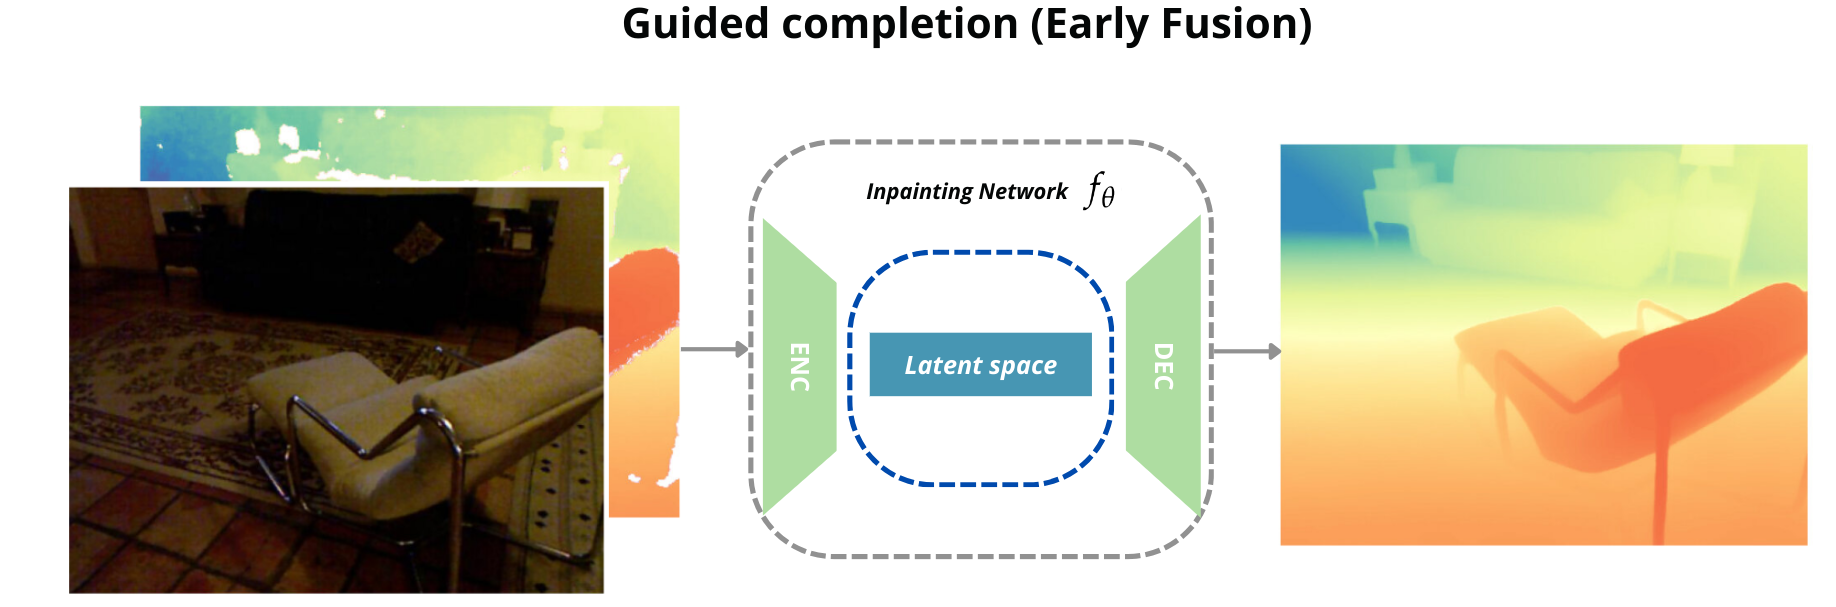
\includegraphics[width=\textwidth]{fig/earlyfusion.png}
    \caption{Esquema de correção guiada com \textit{Early Fusion}.}
    \label{early}
\end{figure}

\begin{figure}[h]
    \centering
    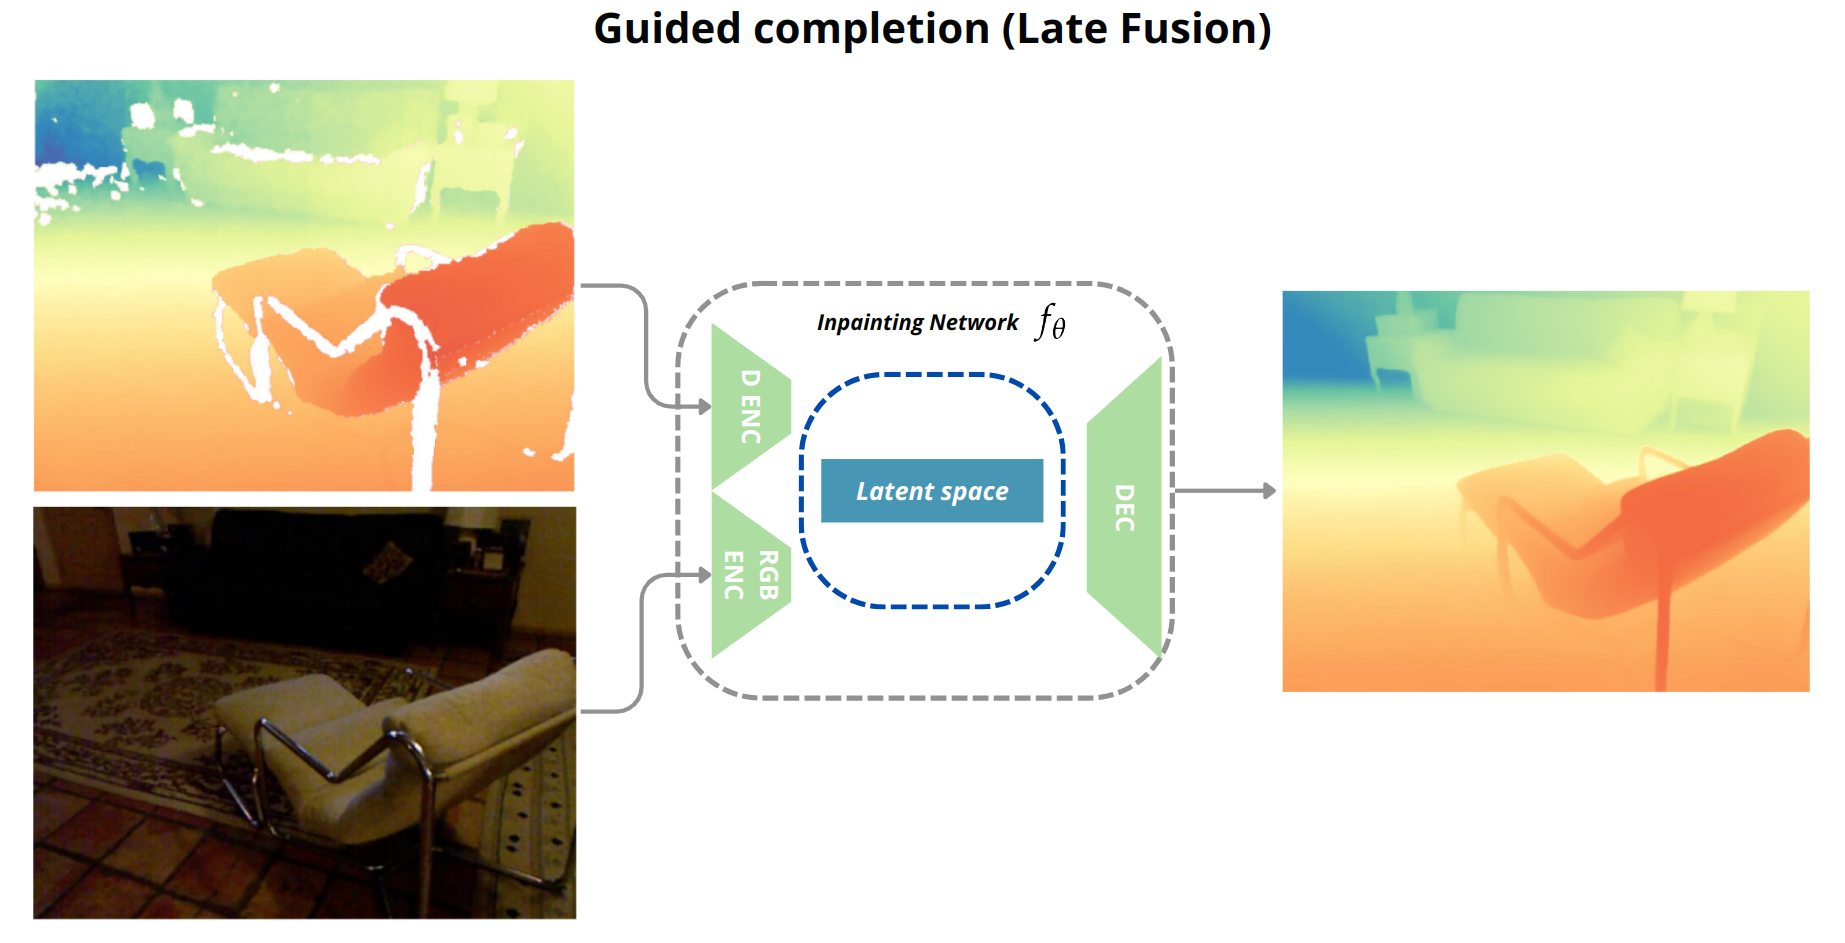
\includegraphics[width=\textwidth]{fig/latefusion.png}
    \caption{Esquema de correção guiada com \textit{Late Fusion}.}
    \label{late}
\end{figure}


\subsection{Large Mask Inpainting}

%Image inpainting is the process of completing or recovering the missing region in the image or removing some objects added to it. 

\textit{Image Inpainting} refere-se ao processo de recuperar regiões faltantes de uma imagem a partir de informação já existente \cite{elharrouss2020image}. Para sintetizar as partes indicadas, é necessário que haja o aprendizado da estrutura global da imagem, sendo imprescindível um vasto campo receptivo na rede neural. Dessa forma, é proposto por \cite{suvorov2022resolution} o sistema LaMa, \textit{Large Mask Inpainting} (Figura \ref{lama}), que é composto por elementos capazes de explorar o campo receptivo apropriado para essa tarefa, sendo eles: i) convoluções rápidas de Fourier (do inglês, \textit{Fast Fourier Convolutions}), ii) o uso de perda perceptual baseada em uma rede de segmentação e iii) uma estratégia de geração de máscaras para treinamento de alta cobertura.

\begin{figure}[h]
    \centering
    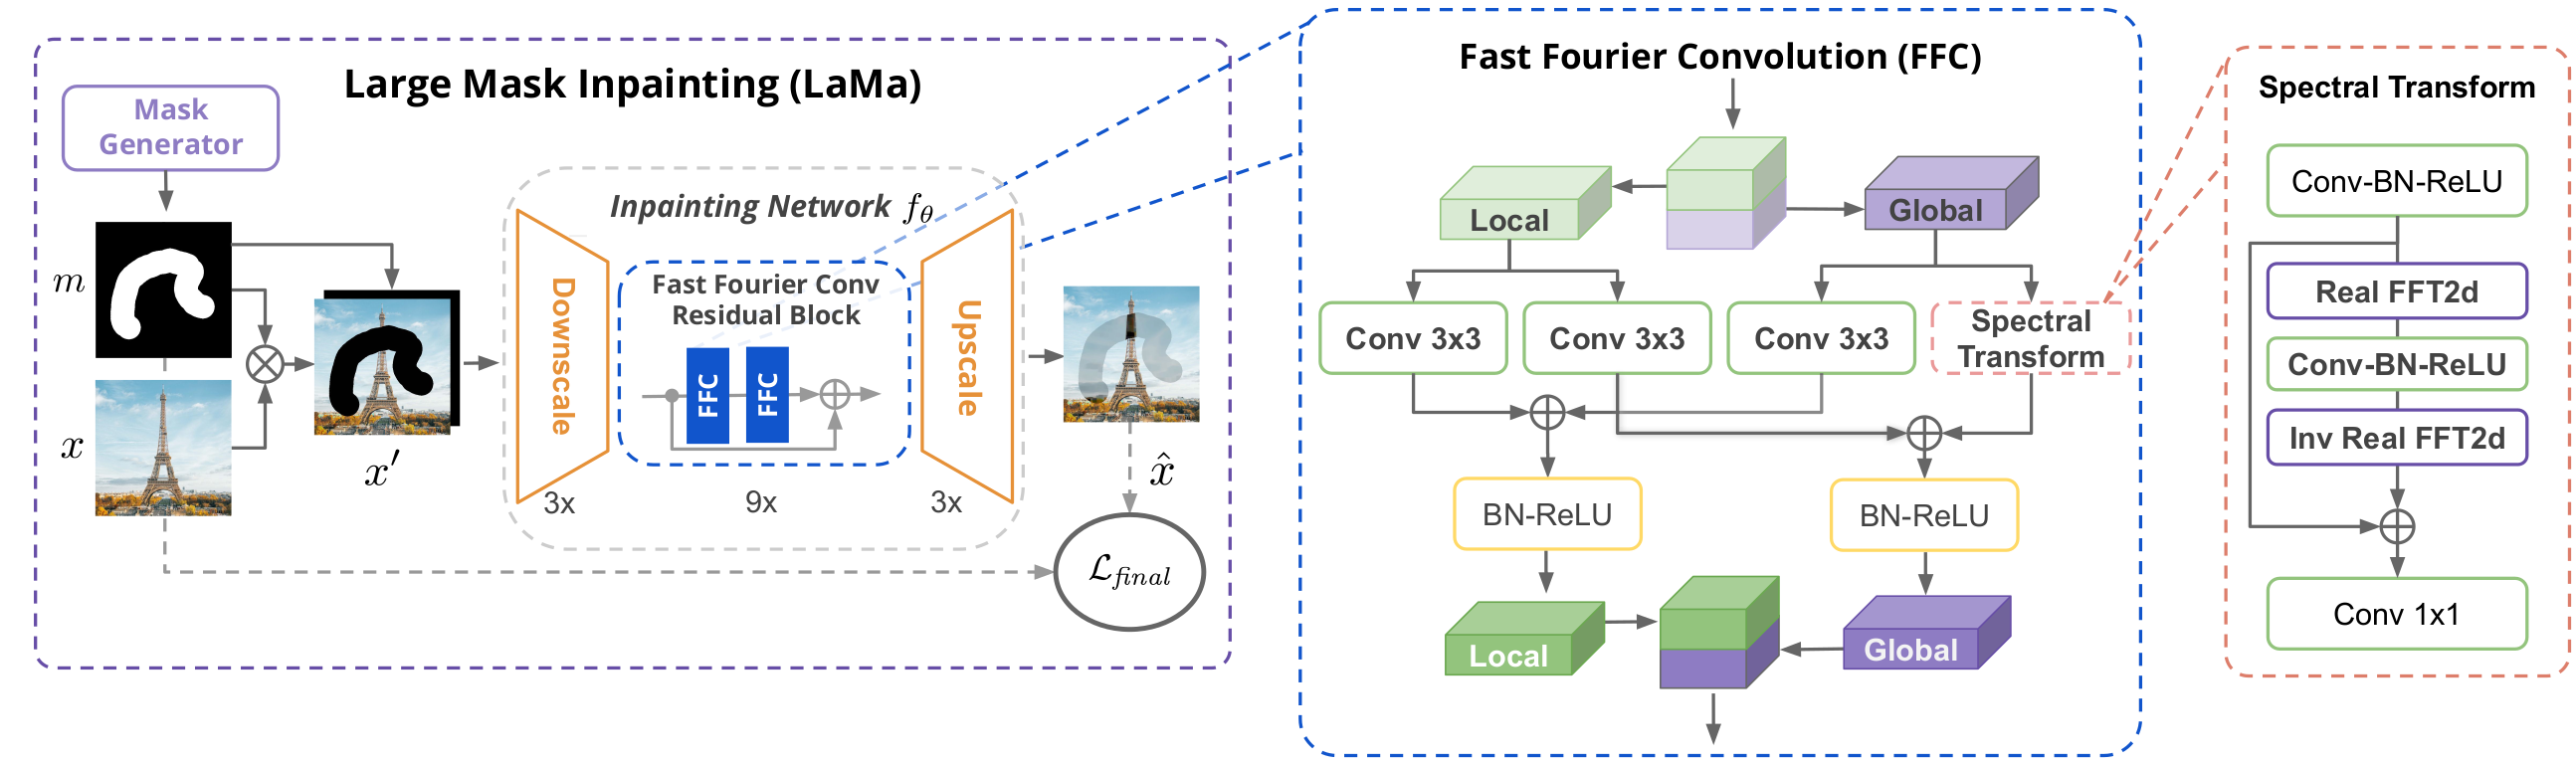
\includegraphics[width=\textwidth]{fig/lama.png}
    \caption{Esquema do método LaMa \cite{suvorov2022resolution}.}
    \label{lama}
\end{figure}

%explain receptive field?




\section{Análise com Aplicação}


\section{Considerações Metodológicas}


    
\chapter{Resultados Preliminares}




% --- -----------------------------------------------------------------
% --- Referencias Bibliograficas. (Obrigatorio)
% --- -----------------------------------------------------------------
    \cleardoublepage
%    \bibliographystyle{acm-2} % abbrv - abnt-num
	%\bibliographystyle{plainnat}
    \bibliography{bibliografia} % arquivo fonte com a bibilografia

% --- -----------------------------------------------------------------
% --- Apendice.(Opcional)
% --- -----------------------------------------------------------------
    \cleardoublepage
    \appendix
    \begin{landscape}
        \chapter{Apêndice A}
\label{appendixA}

...
        % \include{appendixB}
        % \include{appendixC}
        % \include{appendixD}
        % \include{appendixE}
        % \include{appendixF}
        % \include{appendixG}
        % \include{appendixH}
        % \include{appendixI}
        % \include{appendixJ}
        % \include{appendixK}
        %\include{appendixL}
    \end{landscape}
\end{document}